\documentclass[14pt]{matmex-diploma-custom}
\usepackage{enumitem}
\usepackage{amsmath}

% * <svitkovsergey@gmail.com> 13:38:37 13 Dec 2016 UTC+0300:
% ping
\begin{document}
\filltitle{ru}{
    chair              = {Кафедра Системного программирования},
    title              = {Реализация поиска путей с КС-ограничениями в рамках библиотеки YC.QuickGraph},
    type               = {coursework},
    position           = {студента},
    group              = 344,
    author             = {Свитков Сергей Андреевич},
    supervisorPosition = {ст. преп, к. ф-м. н.},
    supervisor         = {Григорьев С.\,В.},
}
\maketitle
\tableofcontents
%\section*{Аннотация}
%	Большинство промышленных языков для написания запросов к графовым базам данных являются регулярными. Но регулярные языки не применимы в ряде задач, поэтому актуальным является создание контекстно-свободного (далее --- КС) языка запросов. Существуют работы по этой теме, но они в основном теоретические. В данной работе рассматривается практическая реализация механизма контекстно-свободных запросов к ориентированным графам с помеченными ребрами для платформы .NET. Результатом работы является библиотека, предоставляющая набор функций для написания КС-запросов к графам. Полученные результаты могут быть применены в проектах, использующих C\# или F\#.

\section*{Введение}
	Разнообразные данные могут быть представлены в виде ориентированного графа с помеченными ребрами. Такая модель имеет широкую область применения и используется в биоинформатике, при реализации графовых баз данных, в социальных исследованиях, semantic web. Работу с такими данными, как правило, выполняют с помощью языков запросов.
	
	Существует множество таких языков, применительно к графовым базам данных наиболее известными являются Gremlin\cite{Gremlin}, Cypher\cite{Cypher}, используемые в графовых базах данных Titan\cite{titan} и Neo4J \cite{neo4j} соответственно. Однако, эти языки являются регулярными, а значит, не могут применяться, например, при разборе генеалогического дерева часто возникает задача поиска потомков общего предка --- поиск последовательностей вида \(parent^nchild^n\). Но строки такого вида не выводимы в языках, задаваемых регулярными грамматиками, однако, могут быть выведены в языке, заданном контекстно-свободной (далее --- КС) грамматикой.  
	
	Существуют работы, предлагающие различные подходы к реализации языков запросов и  процессу исполнения запроса, например \cite{sevon2008subgraph}, \cite{hellings2014conjunctive}, \cite{zhang2016context}, \cite{abiteboul1997regular}, \cite{koschmieder2012regular}. Большая часть перечисленных работ представляет теоретические сведения о реализации, а предлагающие практическую реализацию имеют ограниченный функционал или очень узкую специализацию. Однако класс задач, решение которых возможно с помощью КС-запросов, является обширным, поэтому хотелось бы реализовать инструмент, который имел бы широкую область применения на практике. Для достижения этого необходимо поддерживать различные форматы представления результата запроса, поэтому было принято решение реализовать библиотеку для выполнения КС-запросов к графам, позволяющую представить результат исполнения запроса в нескольких форматах.
	
	Для реализации была выбрана технология .NET. Для неё существует ряд библиотек для работы с графами, например GraphSharp \cite{graphsharp}, Automatic Graph Layout \cite{agl}, но наиболее известной является QuickGraph \cite{quickgraph}, работа над которой прекращена в 2011 году. В лаборатории языковых инструментов JetBrains с 2015 года ведется разработка и поддержка библиотеки YC.QuickGraph \cite{YC.QuickGraph}, за основу которой была взята QuickGraph. Было принято решение использовать её при реализации для работы с графами. В качестве алгоритма для синтаксического анализа графов используется алгоритм синтаксического анализа регулярной аппроксимации на основе GLL\cite{gll}, который в рамках работы \cite{ragRelaxedParsing} был реализован и интегрирован в YaccConstructor \cite{YaccConstructorPage}, \cite{авдюхин2012создание}, \cite{кириленко2013разработка}, \cite{gsv_phd}, \cite{кириленко2013разработка}, \cite{азимов2016syntax}, \cite{ковалев2016реализация}, \cite{полубелова2014генератор} --- исследовательский проект лаборатории языковых инструментов JetBrains, представляющий собой набор инструментов для решения различных задач синтаксического и лексического анализа, реализованный для платформы .NET.
	
\section{Постановка задачи}
    Целью работы является реализация библиотеки для выполнения КС-запросов к графам с использованием .NET, YC.QuickGraph --- в качестве библиотеки для представления графов и YaccConstructor --- для решения задач синтаксического анализа. Результат работы позволяет выполнять КС-запросы к ориентированным графам с помеченными ребрами и представлять результат в виде подграфа, множества путей, кратчайшего пути, КС-отношения (\(R = (N,\, n,\, m)\), где \(N\) --- нетерминал, из которого выводим путь из вершины \(n\) в \(m\). ). 
    
    Для достижения данной цели необходимо решить следующие задачи:
	\begin{itemize}
	    \item разработать алгоритм исполнения запроса с КС-ограничениями;
	    \item спроектировать удобный для пользователя интерфейс задания запросов;
        \item реализовать расширение библиотеки YC.QuickGraph;
        \item опубликовать результат в виде NuGet-пакета.
	\end{itemize}

\section{Обзор предметной области}
	\subsection{Related works}
	В этой секции будут рассмотрены работы, посвященные реализации инструментов для исполнения запросов.
		\subsubsection*{Conjunctive Context-Free Path Queries}
		В данной работе рассматривается построение обобщения существующего регулярного языка запросов к графам с помеченными ребрами CRPQ до КС-языка CCFPQ. Расширение позволяет использовать КС-грамматики вместо регулярных выражений для поиска путей в графе. Предлагаемый в статье алгоритм использует CYK для синтаксического анализа графов. Результатом исполнения запроса является КС-отношение \(R\). К минусам данной работы можно отнести отсутствие практической реализации и возможность представления результата запроса лишь в одном формате.
		\subsubsection*{Subgraph Queries by Context-free Grammars}
		Данная работа рассматривает вопрос о применении КС-запросов в различных задачах биоинформатики. Предложенный в статье подход подразумевает поиск связного подграфа, порождаемого множеством путей, строки из меток на которых выводимы из задаваемой в качестве запроса КС-грамматики. Для синтаксического анализа используется Earley parser \cite{hale2001probabilistic}. Авторами было проведено тестирование алгоритма, предлагаемого в статье, как на случайно сгенерированных, так и на реальных данных. Эксперименты, поставленные на реальных данных, показали, что для графа с максимальной длиной пути, равной 8 вершинам, время работы алгоритма может достигать 250 секунд. Минусами данной работы являются единственный формат представления результата и слишком наивный алгоритм, предлагаемый авторами.
		\subsubsection*{Ослабленный синтаксический анализ динамически формируемых выражений на основе алгоритма GLL}
		В данной работе описыван алгоритм для синтаксического анализа регулярной синтаксической аппроксимации на основе алгоритма GLL, позволяющий проверять выводимость последовательсти меток на ребрах графа, представленных токенами (целочисленными значениями), в задаваемой грамматике. Предложенный в работе алгоритм позволяет обрабатывать входные данные большого размера и может быть использован, например, при поиске подпоследовательностей в метагеномных сборках. Так же была доказана корректность и завершаемость. Следует отметить, что результатом работы алгоритма является лес разбора, представляемый в виде SPPF\cite{SPPF}, который можно отобразить в нужный формат вывода. Учитывая наличие реализации алгоритма для платформы .NET в проекте YaccConstructor, было принято решение использовать результаты автора при реализации.

	\subsection{YaccConstructor}
	    YaccConstructor --- исследовательский проект лаборатории языковых инструментов JetBrains, применимый для исследования и решения различных задач синтаксического и лексического анализа. Проект имеет одноименный инструмент с открытыми исходниками, который включает в себя большое количество компонентов, таких, как язык спецификаций грамматик YARD, алгоритмы для преобразования грамматик, алгоритмы для синтаксического анализа графов и др. Большая часть компонент проекта YaccConstructor реализована для платформы .NET на языке F\#. Поскольку проект имеет модульную архитектуру (рис.\ref{arch}), его компоненты могут быть использованы независимо.
	    
        \begin{figure*}
            \centering
            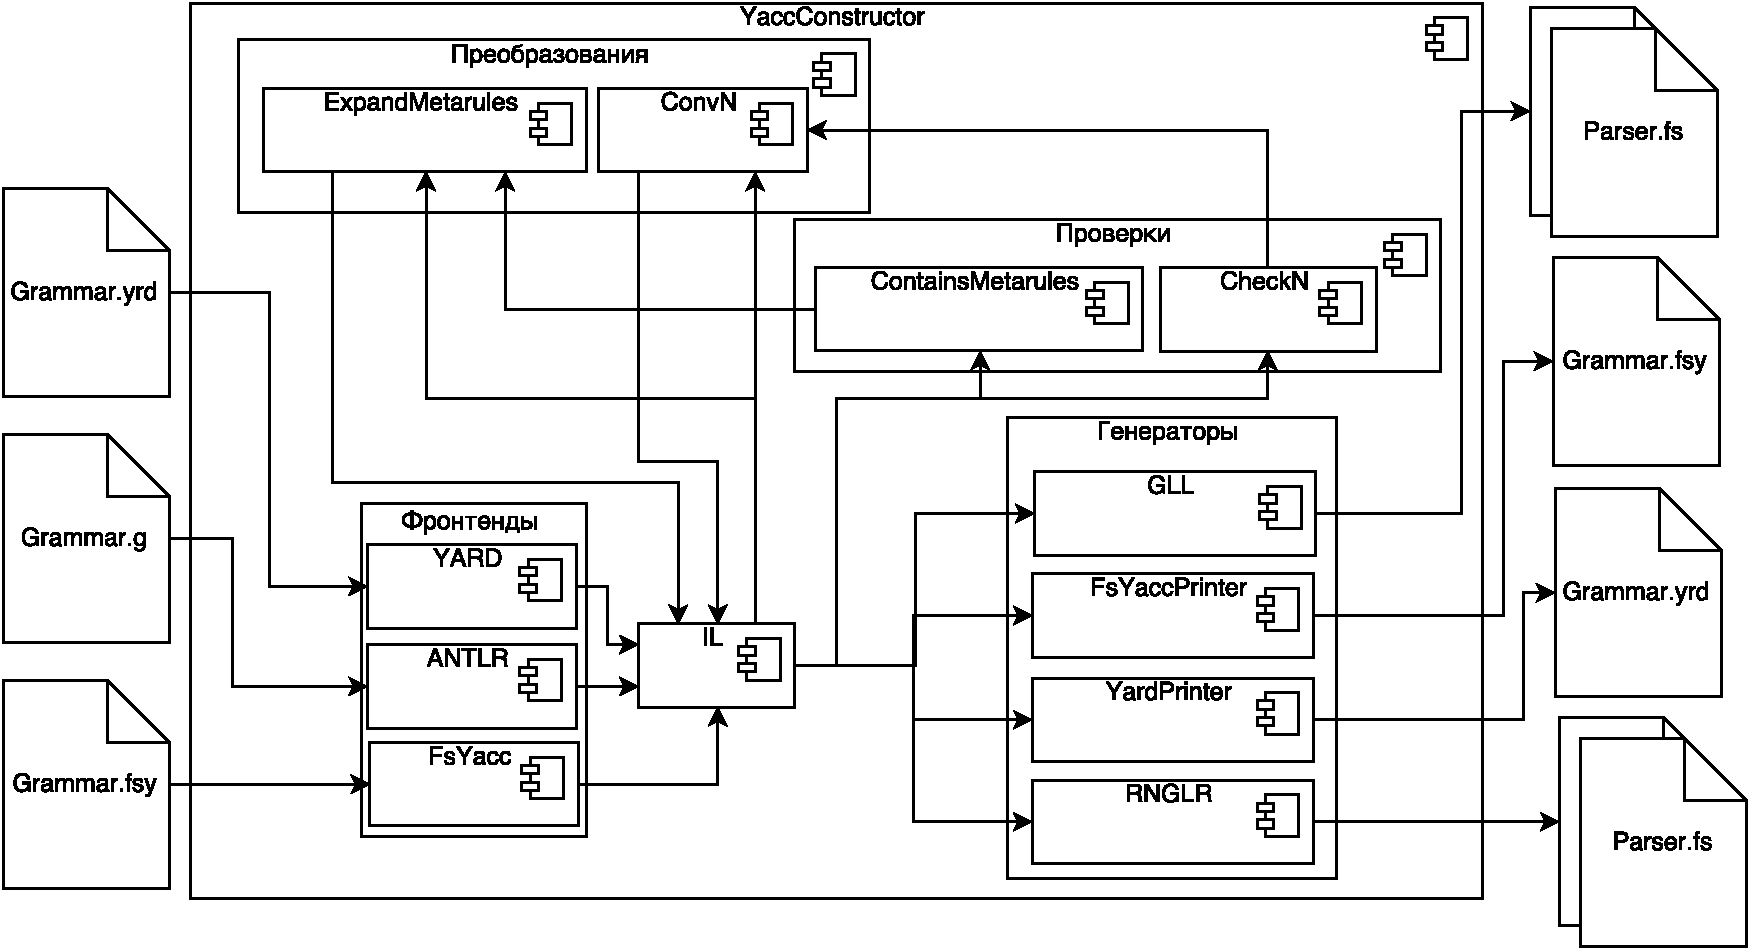
\includegraphics[width=\textwidth]{pics/YCArch.pdf}
            \caption{Архитектура проекта YaccConstructor, заимствована из работы \cite{gsv_phd} \label{arch}}
        \end{figure*}
	    
	    Более подробно рассмотрим YARD, GLLAbstractParser и GLLGenerator. YARD --- язык спецификаций грамматик, позволяющий задавать различные типы грамматик (атрибутные, в нормальной форме Бэкуса-Наура, КС и др.). Так как в рамках данной работы грамматика является запросом, то для его задания будем использовать YARD. GLL --- алгоритм синтаксического анализа, поддерживающий все типы КС-грамматик (в том числе и лево-рекурсивные), кроме того, имеющий асимптотику \(O(n)\) для однозначных граматик и \(O(n^3)\) в худшем случае. GLLGenerator позволяет генерировать парсеры для заданных грамматик (GLLParserSource). GLLAbstractParser позволяет получить из заданного графа и GLLParserSource сжатый лес разбора --- SPPF. SPPF содержит информацию о всех деревьях вывода, что позволяет с помощью различных функций получить результат разбора в нужном формате: в виде КС-отношения, подграфа, множества путей или кратчайшего пути.
	    
	\subsection{YC.QuickGraph}
	    YC.QuickGraph --- проект лаборатории языковых инструментов JetBrains, представляющий собой библиотеку для работы с графами на платформе .NET. YC.QuickGraph не является разработанным с нуля проектом, за его основу взята библиотека QuickGraph \cite{quickgraph}, работа над которой была прекращена в 2011 году. YC.QuickGraph имеет средства для представления графов, различные алгоритмы для них (DFS, BFS, поиск кратчайшего пути и др.). Функионал данной библиотеки планируется использовать для задания пользователем графа и построения вывода в нужном формате.
\section{Реализация}

    \subsection{Архитектура решения}
    
    \begin{figure*}
        \centering
        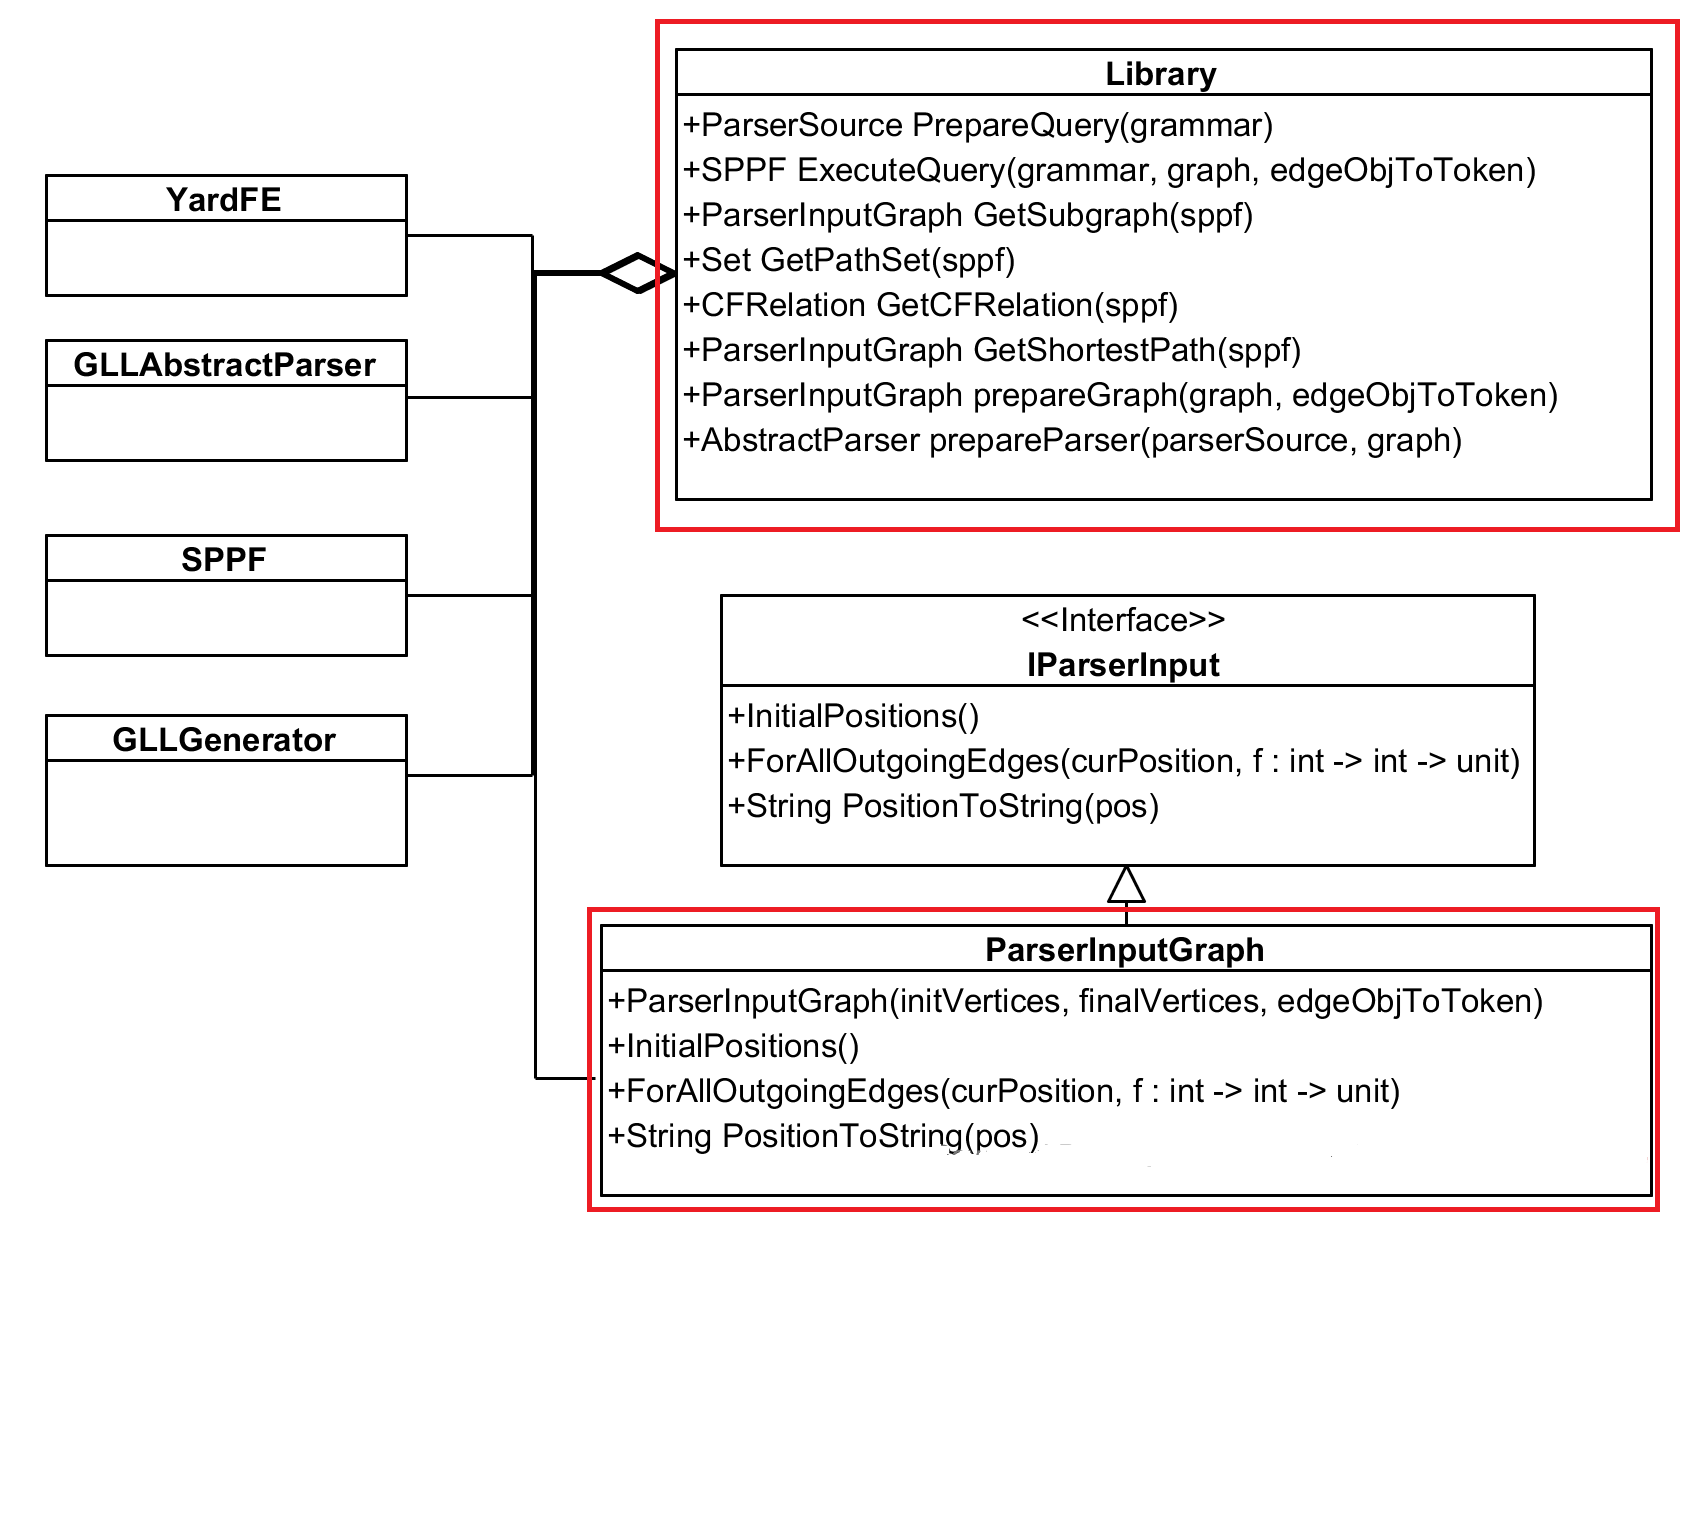
\includegraphics[width=\textwidth]{pics/query.png}
        \caption{Архитектура библиотеки \label{arch_lib}}
    \end{figure*}
    Для предоставления конечному пользователю возможности написания запросов к графу \(G\) и представления результата в одной из нескольких форм была спроектирована архитектура библиотеки (рис.\ref{arch_lib}). При разработке архитектуры были изучены статьи \cite{funcdes1}, \cite{funcdes2}, описывающие основные принципы дизайна функциональных библиотек.
    \begin{figure*}
        \centering
        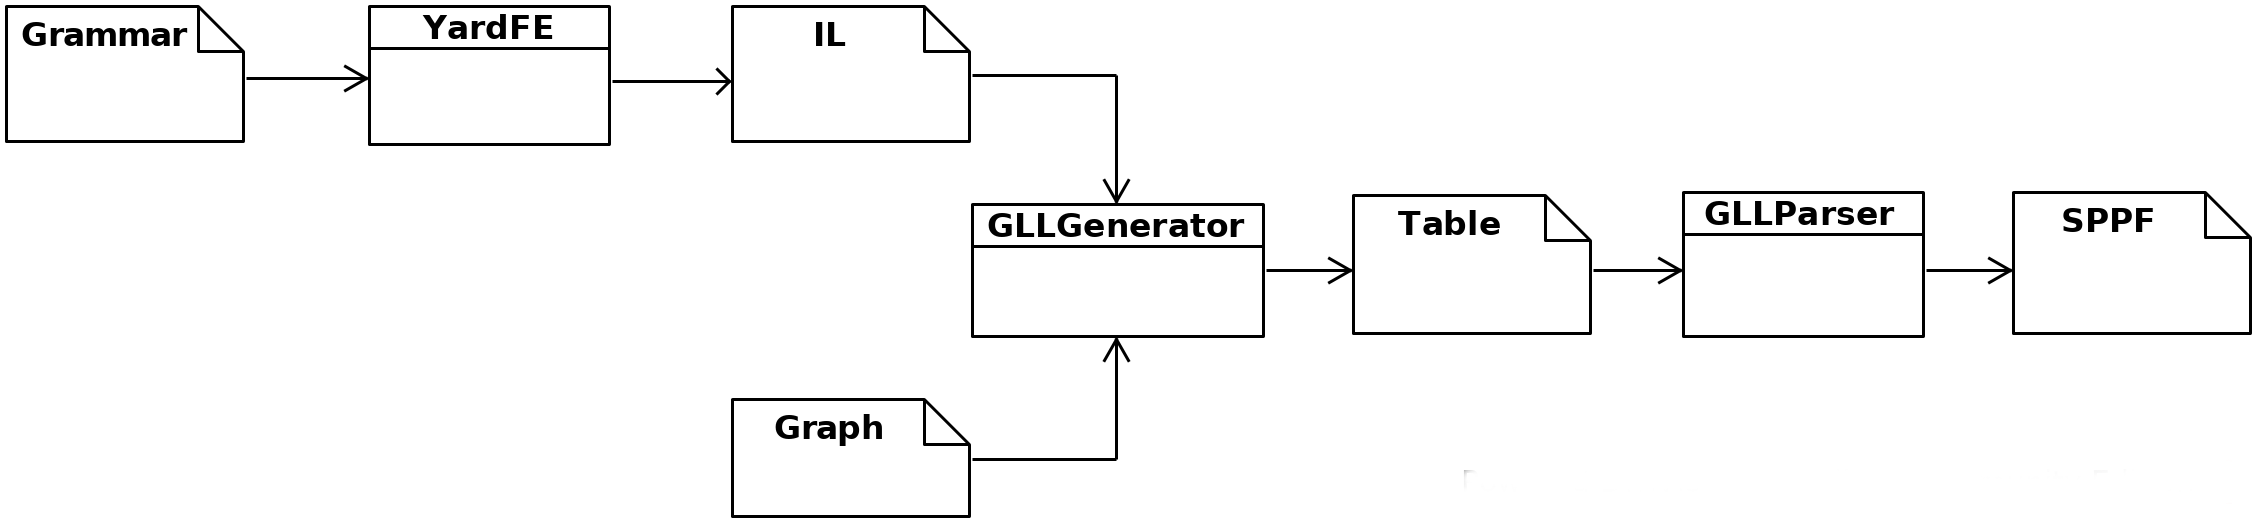
\includegraphics[width=\textwidth]{pics/pipeline.png}
        \caption{Последовательность исполнения запроса \label{pipeline}}
    \end{figure*}
    Пользователь получает возможность написания КС-запросов к задаваемым графам, но само исполнение запроса от него инкапсулировано и производится средствами YaccConstructor и YC.QuickGraph. Существование функций с низким уровнем абстракции позволяет, например, подготовить грамматику для исполнения запроса к нескольким графам. Существование же функций с высоким уровнем абстракции позволит пользователю просто задать запрос к графу и получить результат в желаемом формате. Таким образом, пользователь может комбинировать функции библиотеки, получая инструмент, применимый для решения множества задач.
    
    \subsection{Реализация библиотеки}
    В ходе реализации был решён ряд инженерных задач задач:
    \begin{itemize}
        \item реализовать класс представления графа, поддерживающий преобразование пользовательских объектов в токены;
        \item провести рефакторинг API проекта YaccConstructor;
        \item добавить поддержку генерации ParserSourceGLL для грамматик, заданных в виде строк;
        \item реализовать преобразования SPPF к подграфу, множеству путей, кратчайшему пути и КС-отношению.
    \end{itemize}
    
    Реализация поддержки преобразования пользовательских объектов на рёбрах графа нужна для запуска алгоритма синтаксического анализа на графе, поскольку алгоритм может быть применен только к графам с токенами на рёбрах. Сам процесс преобразования объекта к токену инкапсулирован от пользователя; ему достаточно задать граф в виде одной из реализаций, существующих в библиотеке YC.QuickGraph и функцию, преобразующую объект на ребре в строку. После этого заданный граф преобразуется к нужному формату, а функция \(f: EdgeObject -> token\) получается путём комбинации заданной пользователем функции \(g: EdgeObject -> string\) и функции \(u: string -> token\), получаемой после генерации ParserSourceGLL из задаваемой грамматики с помощью GLLGenerator. После данного преобразования на полученном графе и ParserSourceGLL можно запустить алгоритм синтаксического анализа.
    
    Модуль, в котором было реализовано преобразование грамматики к ParserSourceGLL, был подвергнут рефакторингу. В связи с этим основная функция, выполняющая преобразование грамматики, была разбита на набор функций с более низким уровнем абстракции, что улучшило читаемость и понятность кода и позволило сохранить изначальную функциональность за счёт комбинации полученных функций. Кроме того, была добавлена поддержка генерации ParserSourceGLL из грамматик, заданных строкам.
    
    \subsection{SPPF}
    Для преобразования сжатого леса разбора к желаемым форматам был реализован итератор, позволяющий осуществить обход в ширину. Такой подход используется из-за того, что количество путей в графе, последовательность меток на которых выводима в задаваемом грамматикой языке, может быть бесконечным. Кроме того, обход в ширину позволяет избежать проблем при разборе графов, имеющих циклы. Итератор был написан в lazy-evaluation стиле, то есть результат запроса вычисляется только по требованию пользователя.  
    
    
\section{Заключение}
В ходе работы достигнуты следующие результаты:
\begin{itemize}
    \item изучена предметная область;
    \item проведен обзор статей, связанных с темой работы;
    \item разработана архитектура (рис.\ref{arch_lib}) предлагаемого решения;
    \item реализована библиотека для выполнения КС-запросов к графам;
    \item написаны тесты и документация.
\end{itemize}

\setmonofont[Mapping=tex-text]{CMU Typewriter Text}
\bibliographystyle{ugost2008ls}
\bibliography{coursework}
\end{document}